\chapter{Additional content}


\section{Unity Robotics Hub Overview}

    Before diving into the specifics of establishing the ROS-Unity connection and further develop the project, both tutorials and resources available 
    in the Unity Robotics Hub were studied. This GitHub repository serves as a central hub for tools, tutorials, and documentation tailored for robotic 
    simulation in Unity.

    \subsection{Available Documentation}

    It offers a range of tutorials that are invaluable for setting up and extending ROS-Unity integration, as well as to understand how ROS concepts work inside Unity's environment:
    
    \begin{itemize}
        \item \textbf{ROS–Unity Integration: Initial Setup} - Guides you through the initial steps of setting up communication between ROS and Unity, including package installation and network configuration.
        
        \item \textbf{ROS–Unity Integration: Network Description} - Provides a detailed overview of network settings and offers troubleshooting tips for connectivity issues.
        
        \item \textbf{ROS–Unity Integration: Publisher} - Teaches you how to publish messages from a Unity scene to ROS, with practical examples involving GameObject data.
        
        \item \textbf{ROS–Unity Integration: Subscriber} - Demonstrates how to subscribe to ROS topics in Unity and use the received messages to alter objects in a Unity scene.
        
        \item \textbf{ROS–Unity Integration: Unity Service} - Covers the implementation of ROS services within Unity, allowing Unity to respond to ROS service requests.
        
        \item \textbf{ROS–Unity Integration: Service Call} - Explains how to call external ROS services from Unity, enabling Unity to request data or actions from ROS nodes.
    \end{itemize}
    
    The repository also includes example scripts that correspond to each tutorial.
    
    \section{Establishing the Network Connection}
    After reviewing the Unity Robotics Hub tutorial on network integration, it became clear that establishing a network connection between the Unity and ROS environments was the first crucial step in remote application development. The process involves:
    \begin{itemize}
        \item \textbf{Setting up the network:} Connect the Unity laptop to a Wi-Fi network, then connect the Ubuntu laptop running ROS to the hotspot created by the Unity laptop.
        \item \textbf{Configuring the IP address:} Use the IP address from the Unity laptop within the Unity inspector as shown in Figure \ref{fig:unity_connection}, and in the \texttt{ROSConnection.cs} script to ensure proper communication.
        \item \textbf{Specify the IP Address in ROS Workspace:} A new \textit{.launch} file was created to initialize new nodes, including the \texttt{server\_endpoint} node from the \texttt{ros\_tcp\_endpoint} package, crucial for establishing a proper connection between the ROS and Unity environments. An example of the IP definition in the \textit{.launch} file can be seen below.
    \end{itemize}
    
    \begin{figure}[htbp]
        \centering
        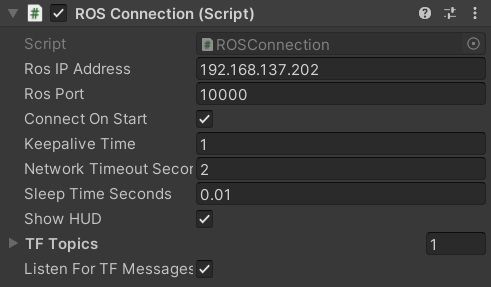
\includegraphics[width=0.5\linewidth]{figs/connection_inspector.png}
        \caption{Unity Connection Inspector}
        \label{fig:unity_connection}
    \end{figure}
    
    % \begin{figure}[htbp]
    %     \centering
    %     \includegraphics[width=\linewidth]{tcp_ip_connection_launch.jpg}
    %     \caption{TCP/IP ROS Node Connection Setup}
    %     \label{fig:tcp_ip_connection}
    % \end{figure}
    \begin{verbatim}
            <arg name="tcp_ip" default="192.168.137.202"/>
            <arg name="tcp_port" default="10000"/>
            
            <node name="server_endpoint" pkg="ros_tcp_endpoint" 
                type="default_server_endpoint.py" args="--wait" output="screen" 
                respawn="true">
                <param name="tcp_ip" type="string" value="$(arg tcp_ip)"/>
                <param name="tcp_port" type="int" value="$(arg tcp_port)"/>
            </node>
    \end{verbatim}
    
    
    This setup is fundamental for the Unity environment to interact effectively with ROS, allowing for real-time data exchange and control commands to be sent between the two systems. Further details are available in the Unity Robotics Hub tutorial on \href{https://github.com/Unity-Technologies/Unity-Robotics-Hub/blob/main/tutorials/ros_unity_integration/network.md}{ROS-Unity integration}.


    \section{ROS Message Generation}
    
    After establishing the communication between ROS and Unity, as well as the other basic communication channels—publishers, subscribers, and services, the next step was to customize these components to handle the specific types of messages required for this project.
    
    \subsection{Adapting to Specific Message Types}
    
    To begin, I revisited the previously mentioned GitHub repositories for the UR10e robot, specifically focusing on identifying which ROS nodes and topics were critical for my Unity-ROS integration. This involved:
    \begin{itemize}
        \item \textbf{Identifying Key Nodes and Topics:} The primary focus was on 
        % the \texttt{/joint\_states} topic,
        finding which topic is responsible for publishing the current state of the robot’s joints.
        \item \textbf{Message Subscription and Retrieval:} With guidance from my supervisors, I determined that subscribing to the \texttt{/joint\_states} topic would be essential for retrieving real-time data about the robot's joint positions.  This topic uses the \texttt{sensor\_msgs/JointState} message type, a standard message in ROS that provides the positions, velocities, and efforts of the robot's joints. It is well-documented and includes the necessary fields for capturing joint states. This message type is part of the broader \texttt{common\_msgs/sensor\_msgs} package, which is available on the \href{https://wiki.ros.org/sensor_msgs}{ROS wiki} and in the \href{https://github.com/ros/common_msgs/tree/noetic-devel/sensor_msgs/msg}{sensor\_msgs GitHub repository}.
    \end{itemize}
    
    \subsection{ROS-TCP Connector and C\# Message Generation}
    
    To correctly handle the \texttt{sensor\_msgs/JointState} messages within Unity, it was necessary to generate corresponding C\# classes. This process, which is detailed in the \href{https://github.com/Unity-Technologies/ROS-TCP-Connector/blob/main/MessageGeneration.md}{ROS-TCP Connector documentation}, involves:
    \begin{enumerate}
        \item \textbf{Generating C\# Message Classes:} By following the steps provided in the documentation, I was able to generate the necessary C\# JointState class that represent the corresponding ROS message, as depicted in the figure \ref{fig:unityjoint_state_message}. This step was crucial for storing and manipulating the joint state data within the Unity environment.
        \begin{figure}
        \centering
        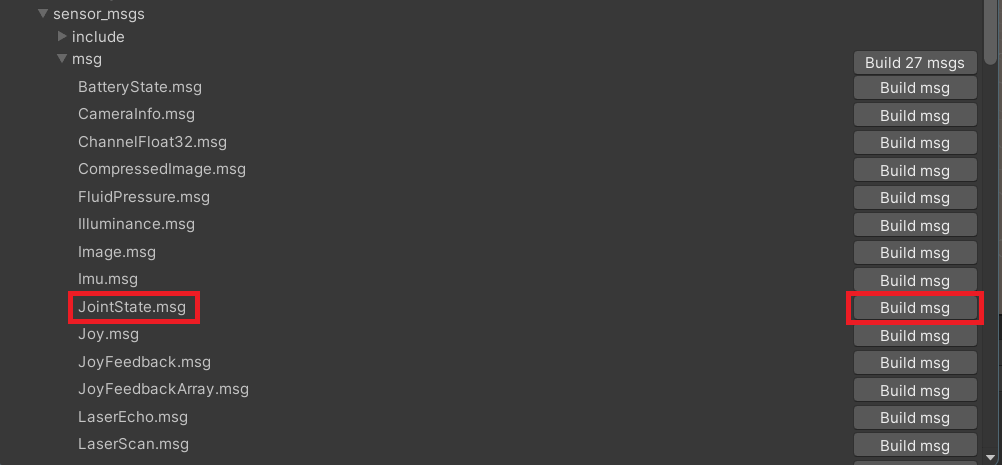
\includegraphics[width=0.75\linewidth]{figs/unityjoint_state_message.png}
        \caption{JointState message generation in Unity, corresponding to the desired ROS message}
        \label{fig:unityjoint_state_message}
        \end{figure}
        \item \textbf{Compiling and Verifying the Message Classes:} After generating the message classes, I compiled them in the Windows environment, ensuring they matched the expected structure as described in the UnityRoboticsTutorial repository. This process took some time to fully understand, but was critical for the successful integration of ROS data into Unity.
    \end{enumerate}